%%%%%%%%%%%%%%%%%%%%%%%%%%%%%%%%%%%%%%%%%
% Large Colored Title Article
% LaTeX Template
% Version 1.1 (25/11/12)
%
% This template has been downloaded from:
% http://www.LaTeXTemplates.com
%
% Original author:
% Frits Wenneker (http://www.howtotex.com)
%
% License:
% CC BY-NC-SA 3.0 (http://creativecommons.org/licenses/by-nc-sa/3.0/)
%
%%%%%%%%%%%%%%%%%%%%%%%%%%%%%%%%%%%%%%%%%

%----------------------------------------------------------------------------------------
%  PACKAGES AND OTHER DOCUMENT CONFIGURATIONS
%----------------------------------------------------------------------------------------

\documentclass[DIV=calc, paper=a4, fontsize=11pt, twocolumn]{scrartcl}   % A4 paper and 11pt font size

\usepackage{lipsum} % Used for inserting dummy 'Lorem ipsum' text into the template
\usepackage[english]{babel} % English language/hyphenation
\usepackage[protrusion=true,expansion=true]{microtype} % Better typography
\usepackage{amsmath,amsfonts,amsthm} % Math packages
\usepackage[svgnames]{xcolor} % Enabling colors by their 'svgnames'
\usepackage[hang, small,labelfont=bf,up,textfont=it,up]{caption} % Custom captions under/above floats in tables or figures
\usepackage{booktabs} % Horizontal rules in tables
\usepackage{fix-cm}   % Custom font sizes - used for the initial letter in the document

\usepackage{listings}



\usepackage{sectsty} % Enables custom section titles
\allsectionsfont{\usefont{OT1}{phv}{b}{n}} % Change the font of all section commands

\usepackage{fancyhdr} % Needed to define custom headers/footers
\pagestyle{fancy} % Enables the custom headers/footers
\usepackage{lastpage} % Used to determine the number of pages in the document (for "Page X of Total")

\usepackage[pdftex]{graphicx}
\usepackage{pgfplots}
\usepackage{hyperref}
\usepackage{amsmath}



% Headers - all currently empty
\lhead{}
\chead{}
\rhead{}

% Footers
\lfoot{}
\cfoot{}
\rfoot{\footnotesize Page \thepage\ of \pageref{LastPage}} % "Page 1 of 2"

\renewcommand{\headrulewidth}{0.0pt} % No header rule
\renewcommand{\footrulewidth}{0.4pt} % Thin footer rule

\usepackage{lettrine} % Package to accentuate the first letter of the text
\newcommand{\initial}[1]{ % Defines the command and style for the first letter
\lettrine[lines=3,lhang=0.3,nindent=0em]{
\color{DarkGoldenrod}
{\textsf{#1}}}{}}

%----------------------------------------------------------------------------------------
%  TITLE SECTION
%----------------------------------------------------------------------------------------

\usepackage{titling} % Allows custom title configuration

\newcommand{\HorRule}{\color{DarkGoldenrod} \rule{\linewidth}{1pt}} % Defines the gold horizontal rule around the title

\pretitle{\vspace{-30pt} \begin{flushleft} \HorRule \fontsize{24}{24} \usefont{OT1}{phv}{b}{n} \color{DarkRed} \selectfont} % Horizontal rule before the title

\title{Real-time Sound Feature Construction and Detection for Game Input } % Your article title

\posttitle{\par\end{flushleft}\vskip 0.5em} % Whitespace under the title

\preauthor{\begin{flushleft}\large \lineskip 0.5em \usefont{OT1}{phv}{b}{sl} \color{DarkRed}} % Author font configuration

\author{Ben Schwab, } % Your name

\postauthor{\footnotesize \usefont{OT1}{phv}{m}{sl} \color{Black} % Configuration for the institution name
Duke University, Math 361S Spring 2014 % Your institution

\par\end{flushleft}\HorRule} % Horizontal rule after the title

\date{5/2/2014} % Add a date here if you would like one to appear underneath the title block

%----------------------------------------------------------------------------------------

\begin{document}

\maketitle % Print the title

\thispagestyle{fancy} % Enabling the custom headers/footers for the first page

%----------------------------------------------------------------------------------------
%  ABSTRACT
%----------------------------------------------------------------------------------------


% The first character should be within \initial{}
\initial{T}\textbf{his paper investigates a system to process and identify a set of sound events (specifically whistles and snaps) for use as input to a video game. The environment of a game provides unique constraints that requires real time feature generation and recognition. The paper begins with a brief introduction of sound processing, a background on the Discrete Fourier Transform, and its practical implementation, the Fast Fourier Transform. Then there is a description of the decision pipeline including the audio features generated on the audio samples and the expected features of snaps and whistles.}

%----------------------------------------------------------------------------------------
%  ARTICLE CONTENTS
%----------------------------------------------------------------------------------------
\tableofcontents

\section{Introduction}

\par The last five years have marked enormous change in how people interact with video games. From the explosion of touch-based smart phone games to more complex technologies like Microsoft's Kinect, users are interacting with games in more natural and immersive manners. Sound based input has historically been a challenging problem because of the computational complexity of obtaining near $100\%$ accuracy required for an enjoyable video game experience. In this paper I propose a limited set of sound input actions: whistles and snaps. The small set allows faster and more accurate recognition than traditional speech based input. In addition, the choice of this input set allows a surprising amount of user control. As whistles have a distinct pitch, they can be mapped to a two-dimensional scalable input (think of a joystick that can move only up and down). Snapping is a binary input that is most similar to pushing a button on a controller.
\par The primary focus of this paper is the construction of a JavaScript library which will generate ``whistle'' and ``snap'' events. The paper can also be used as a frame to introduce the basics of the DFT and it's application to Digital Sound Processing. In the \textbf{Discussion} section, I discuss a proof of concept game where the library is used. Currently the game, WhistleHero, can be accessed on \textbf{benschwab.github.io}. The entire code is available at \textbf{https://github.com/ BenSchwab/BenSchwab.github.io}.

\subsection{Identification Pipeline overview}
\begin{figure}[h]
\centering
\includegraphics[width=90mm]{figures/HighLevelPipeline.png}
\caption{High level overview of the identification pipeline.}
\label{overflow}
\end{figure}
A major challenge of this project is establishing a pipeline which can both analyze sound and determine when snaps and whistles occur. The identification pipeline (see figure one) starts as soon as a stream of audio is established from a user's laptop microphone. The stream is processed in segments in a local context. A set of features such as energy, fundamental frequency, flatness and envelope shape are attached to the sample during this stage. Due to the real-time restriction of generating input for a video game, instantaneous features in both the time and frequency domain are primarily used, however, the pipeline design allows for global features to be analyzed, albeit in a limited manner.
\par To get the frequency information of the input sound (used for generation of the spectral features of the sound sample) I use the \textbf{Discrete Fourier Transform}, specifically, the optimized \textbf{Fast Fourier Transform}  which can switch a signal between frequency and time representations.
\par Finally, after all the features of a sample have been generated, the similarity of the sample is compared to expected feature sets of whistles and snaps which I established by generating features on a controlled dataset. Using a binary perceptron model, if a similarity threshold is met, a sound event is emitted.

%------------------------------------------------



%------------------------------------------------

\section{Background}
In this section I give a background on digital sound in the time and frequency domains. Experienced readers can skip to section 2.3 where a background on the constraints of a real time JavaScript sound detection engine are discussed.
\subsection{Digital Sound and the Time Domain}
Sound is a longitudinal wave of pressure variations. Figure 2 gives a visual representation of a sound pressure wave. At an instant in time, the ear perceives the wave at some pressure level. A plot of the intensity over time would be a continuous function (commonly written as $s(t)$) recorded by some target such as an ear or microphone. The WebAudioApi (used in this paper) normalizes the pressure measurements to be between -1 and 1, where -1 represents low pressure and 1 represents high pressure. This system is known as \textbf{Pulse Code Modulation} or \textbf{PCM}.

\begin{figure}[h]
\centering
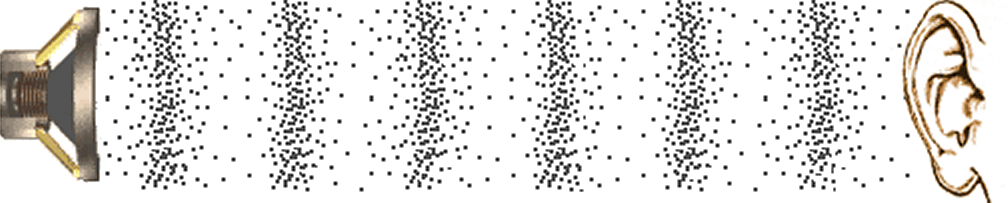
\includegraphics[width=80mm]{figures/pressure_wave.png}
\caption{Sound is the result of high pressure / low pressure variations. [Smuss, 2013]}
\label{overflow}
\end{figure}

\par A microphone records sound samples at a fixed sampling rate, $ f_s = 1/t_s $ where $t_s$ is how often the sound is sampled. In this project we record at the standard sampling rate of
 $44,100Hz$ or roughly a value every $t_s =0.02$ milliseconds. This process of converting a continuous signal into a set of discrete values is known as \textbf{quantization}. Figure 3 illustrates the quantization process.

 \begin{figure}[h]
\centering
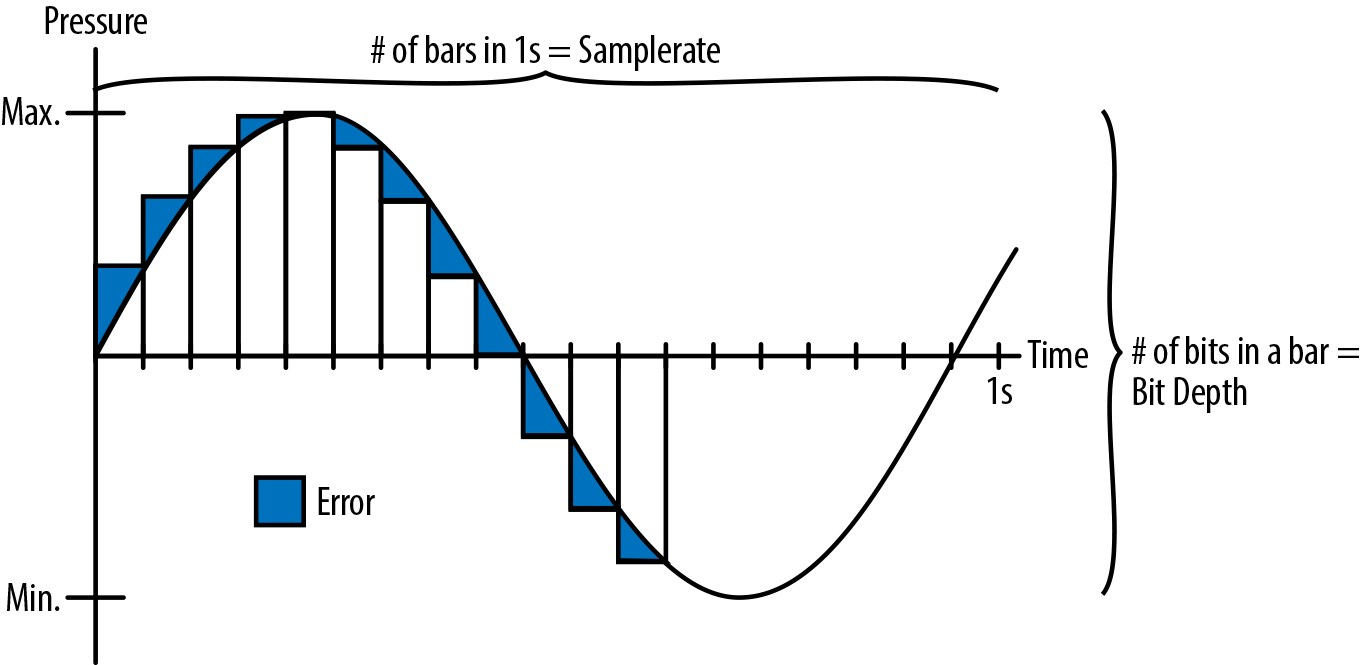
\includegraphics[width=75mm]{figures/quantization.png}
\caption{The quantization process which transforms a continuous sound signal into a discrete array of amplitude values.[Smuss, 2013]}
\label{overflow}
\end{figure}

\begin{figure}[h]
\centering
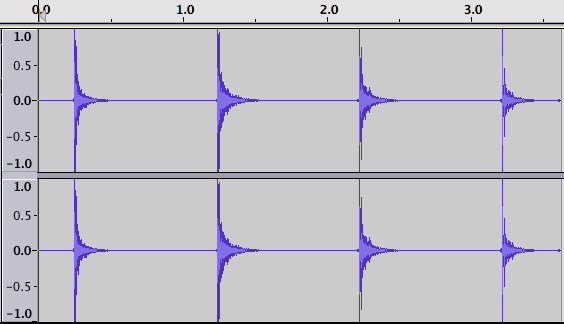
\includegraphics[width=60mm]{figures/snap_timedomain.png}
\caption{The time domain of four finger snaps.}
\label{overflow}
\end{figure}

These sampled signal values represent the signal in the \textbf{time domain}. The time domain information of four snaps is shown in Figure 4.
\subsection{Frequency Domain}
Sound can be modeled as a periodic function in the time domain. Therefore, there is thus an intimate relationship between sound and trigonometric functions. For example, a steady tone can be generated by pressure values in the time domain which follow the pattern of a sine wave. Depending on the period of the wave, we hear a different ``pitch'' (or, more appropriately, frequency). In a sense, the faster packets of high pressure hit one's ear, the higher the pitch one hears.
\par  In the case of a pure sine wave, we could represent the signal in a new \textbf{Frequency Domain} under which it would take on a set of frequency values represented by the function: $f(x_f)$. This function indicates how much of a certain frequency is contained in the sound wave. For the case of a simple tone wave, in the frequency domain it would have a high peak at one frequency, $x_f$, and be zero everywhere else. See Figure 5.

\begin{figure}[h]
\centering
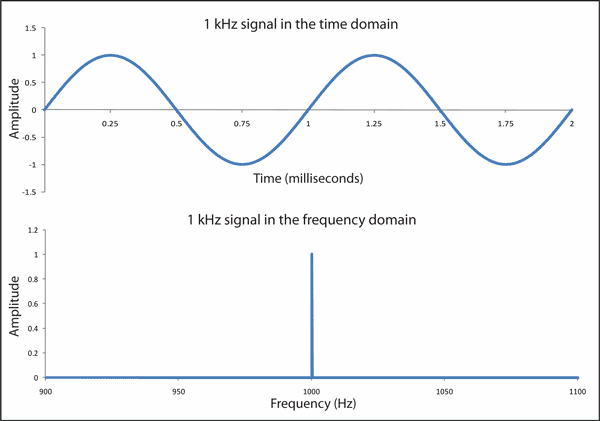
\includegraphics[width=60mm]{figures/twodomains.png}
\caption{An a simple tone converted between time and frequency domains.[Smuss, 2013]}
\label{overflow}
\end{figure}

\par A sound that can be modeled as a single sinusoid sounds very synthetic. The sounds we hear every day are complex, and fittingly, the signal that represents those sounds look very complex (note the complexity of snaps in Figure 4).

\begin{figure}[h]
\centering
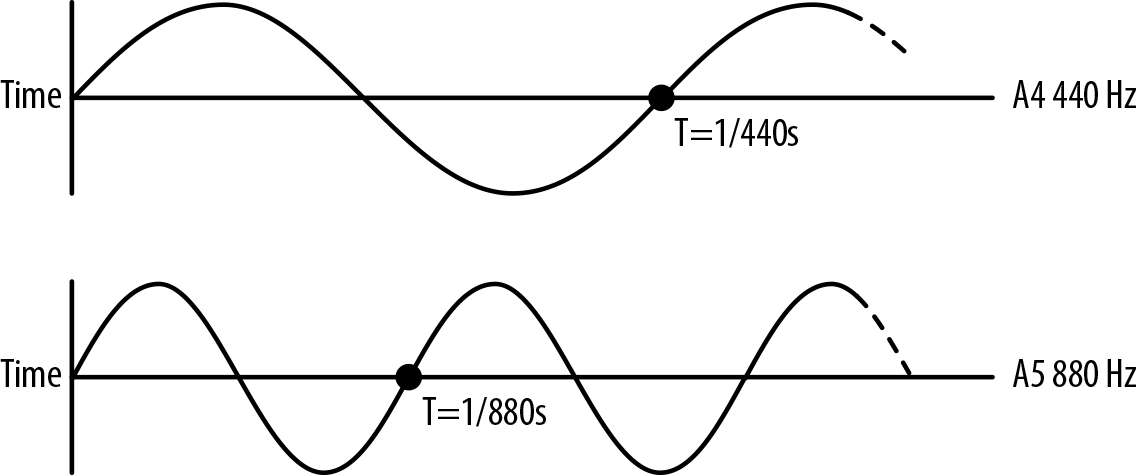
\includegraphics[width=90mm]{figures/PitchGraph.png}
\caption{Two different pure-tone pitches in the time-domain.[Smuss, 2013]}
\label{overflow}
\end{figure}

\begin{figure}[h]
\centering
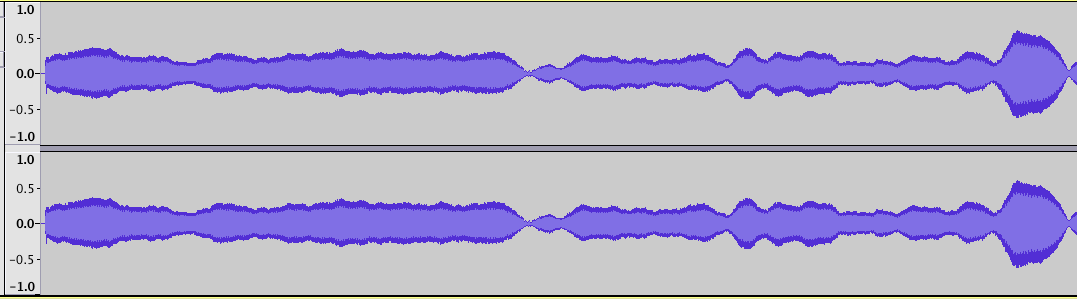
\includegraphics[width=80mm]{figures/whistletimedomain.png}
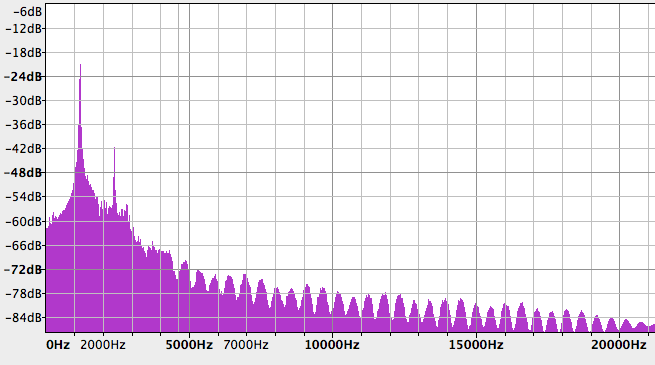
\includegraphics[width=80mm]{figures/frequencydomainwhistle.png}
\caption{A constant whistle signal in the time domain (top) and in the frequency domain(bottom). The frequency domain clearly reveals that the whistle has a prominent frequency component at approximately 1200 Hz. Indeed, this is the pitch of the whistle. }
\label{overflow}
\end{figure}

   One of the most important discoveries for the field of signal processing was made by Joseph Fourier whose titular \textbf{Fourier Transform} allows \textit{any} signal to be switched between its time and frequency representation. More specifically, the Fourier Transform states that any function can be represented to an arbitrary degree of accuracy by the sum of cosine and sine functions of varying amplitudes and frequencies. Thus, a complex sound can be represented as the sum of a series of synthetic ``basis'' sounds which combine to make rich noise.



  \par As Figure 7 shows, very useful information about a sound signal is revealed in the frequency domain. The whistle in Figure 7 demonstrates a characteristic shape in the frequency domain, with a distinctive peak at the pitch of the whistle. Generation of features in the frequency domain is known as \textbf{Spectral Analysis}. The Identification Pipeline also analyzes the input sound in the time domain. This is known as \textbf{Temporal Analysis}.

\subsection{JavaScript Game Engine Constraints}
JavaScript presents a unique environment to preform active sound input detection due to it's single threaded nature. The following discussion will be at a high-level intending only to frame some of the challenges of using JavaScript to handle Sound Input. Figure 8 shows a representation of JavaScript's single thread. (Sound recording is handled natively through Chrome off the main thread, thankfully.) We receive chunks of approximately 46 milliseconds of sound. Thus, there are 46 milliseconds to fully process the last 46 milliseconds of sound. However, in this 46 milliseconds the game must also render on screen. It does this approximately every 16.6 milliseconds to achieve a frame rate of 60fps. The game could use some arbitrary portion of the gap between successive animation calls to update it's logic, and render itself. An input engine should allow the maximum about of time possible to be given to the game to compute complex graphical situations.
\par Thus, the engine is written in such a manner that it can detect if the queue of incoming sound is building up. If so it increases its \textbf{hop size} by a factor of 2, effectively cutting processing time in half. See section 4.1.1 for a more in depth explanation of hop size, and the input process.
\begin{figure}[h]
\centering
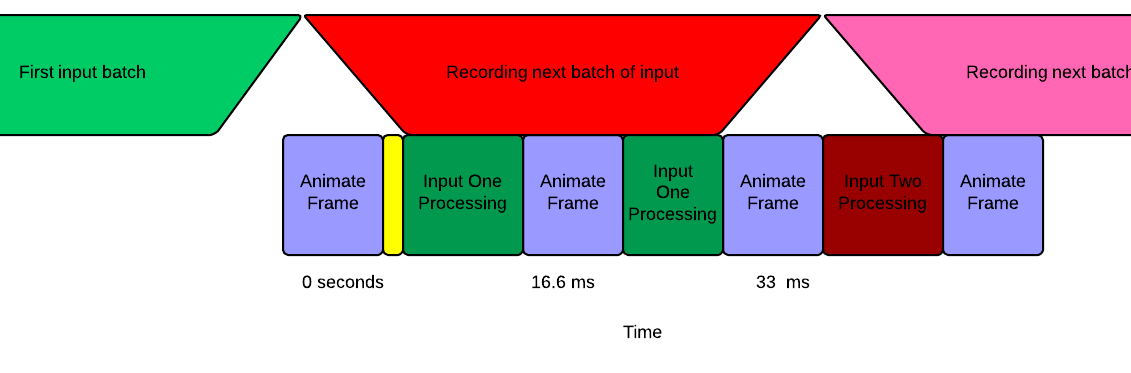
\includegraphics[width=80mm]{figures/JavascriptEventLoop.png}
\caption{JavaScript is single threaded. The sound processing must occur in the windows left open in the game.}
\label{overflow}
\end{figure}

\par The take away from this section is: the Sound Input Engine is guaranteed to  have \textbf{46 ms} of input lag, and often less. The engine will adapt to a heavily computational game by decreasing the number of times a sample is processed, which comes at the cost of increasing false negatives.


\section{General Methods}
The primary numerical method of this paper is the Fast Fourier Transform, or FFT. For readers unfamiliar with the FFT, I start this section with a mathematical derivation of the Discrete Fourier Transform, or DFT, the method which the FFT optimizes. Experienced readers can skip to section 4 where the pipeline and identification methods are covered in detail.
\subsection{Theory of Fourier Transform}
\textsubscript{Adapted from [Sauer, 2012]}
\subsubsection{Mathematical Derivation}

While not strictly necessary for Fourier Transform to function, I will begin the explanation of the DFT by discussing Euler's formula which vastly simplifies the representation of the transform and gives a beautiful geometric interpretation:

\begin{align}
e^{i\theta} = cos(\theta) + isin(\theta)
\end{align}

Equation 1, Euler's formula, is an elegant way to express the set of complex numbers with magnitude equal to one. Figure 9 shows the mapping between the unit circle in the complex plane and Euler's formula.

\begin{figure}[h]
\centering
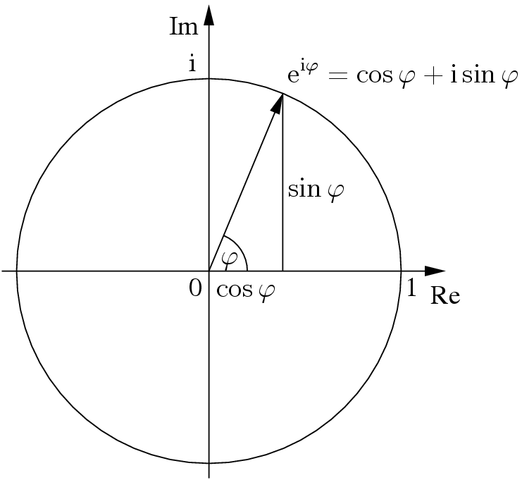
\includegraphics[width=40mm]{figures/EulersFormula.png}
\caption{The connection between the unit circle in the complex plane and Euler's formula. }
\label{overflow}
\end{figure}


Multiplying numbers from Euler's formula is as simple as adding the exponents.

\begin{align}
e^{i\theta}e^{i\gamma} = e^{i(\theta+\gamma)}
\end{align}
Appropriately, this has the geometric meaning that the product of two complex numbers on the unit circle, is another complex number on the unit circle with the new angle the sum of the angles of the factors.
\par We now consider the complex numbers, $z$, on the unit circle such that $z^n = 1 $. Such complex numbers are known as the \textbf{$n$th roots of unity}. If a complex number z is $n$th root of unity, but not a $k$th root of unity for any $k<n$, we consider it be a \textbf{primitive nth root of unity}. Intuitively, this means if we were to raise this angle to a power, the first time it would equal one is at the $n$th power. Imagine dividing the circle in $n$ equal pieces, where each line represents a root of unity. Figure 10 demonstrates this with $n=8$. As multiplication correlates to addition of angles, the only way a root of unity can be primitive is if the GCD of its index and $n$ is one.

\begin{figure}[h]
\centering
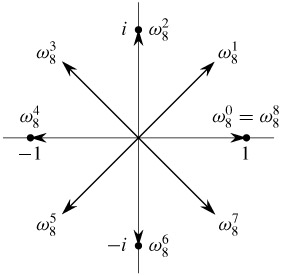
\includegraphics[width=40mm]{figures/eighthroots.jpg}
\caption{The eighth roots of unity. }
\label{overflow}
\end{figure}


 It is standard to let $\omega = e^{-i2\pi/n}$ which is always a $n$th root of unity as, following the previous argument, $\omega^k = e^{-ik2\pi/n}$ whose index is n-1, is guaranteed to be relatively prime with n.


The first important statement for the Discrete Fourier Transform is that if $\omega$ is an $n$th primitive root of unity then

\begin{align}
1 + \omega + \omega^2 + \omega^3 + ... + \omega^{n-1} = 1.
\end{align}

This is can be verified with the telescoping sum:

\begin{align}
(1 - \omega)(1 + \omega + \omega^2 + \omega^3 + ... + \omega^{n-1}) = 1 - \omega^n = 0.
\end{align}

As the left factor is not equal to zero, the right factor must be 0. \par The following equation arrives from the fact that $\omega^n = 1$ as it is a $n$th root of unity. Thus raising $\omega$ to multiples of $n$ must also be one:

\begin{align}
1 + \omega^n + \omega^{2n} +  ... + \omega^{n(n-1)} = 1 + 1  ...+ 1 = n.
\end{align}

We can combine (4) and (5) to get:


\begin{align}
\sum_{j=0}^{n-1}\omega^{jk} = \left\{
   \begin{array}{ll}
      n  & \mbox{if } k/n \mbox{ is an integer }\\
      0 & \mbox{ otherwise }
   \end{array}
\right.
\end{align}

The proof follows below: \\

For any k we can write k as $k = m*n +r $ where $r < n$. Thus we can write $\omega^{jk}$ as: $$\omega^{j*(m*n+r)} = \omega^{jmn}\omega^{jr} $$ However, $\omega^{jmn}=1$ by definition of $\omega$ being a $n$th root of unity. If $n$ divides $k$ then $\omega^{jr} = 1$ as $r=0$. In this case, the sum becomes $\sum_{j=0}^{n-1}1=n$ If not then the sum becomes $\sum_{j=0}^{n-1}\omega^{jr}$ for some $r<n$. However, we can use an altered telescope sum, as done in equation 4:
\begin{align}
(1 - \omega^r)(1 + \omega^r + \omega^{2r} + \omega^{3r} + ... + \omega^{r*(n-1)}) = 1 - \omega^n = 0.
\end{align}
Again, as $(1 - \omega^r)$ can not equal zero due to $\omega$ being a primitive root of unity, the right factor must equal 0. Hence, we conclude (6) is valid.


\par Using this knowledge we can now define \textbf{Discrete Fourier Transform}:

\begin{align}
y_k = \frac{1}{\sqrt{n}}\sum_{j=0}^{n-1}x_j\omega^{jk}.
\end{align}

It is useful to define the Fourier Matrix, $F_{n}$, of degree n as:

\begin{align}
 (1/\sqrt n)
 \begin{pmatrix}
  \omega^0 & \omega^0 & \omega^0 & \cdots & \omega^0 \\
  \omega^0  & \omega^1 & \omega^2 &  \cdots &  \omega^{n-1} \\
   \omega^0  & \omega^2 & \omega^4 &  \cdots &  \omega^{2(n-1)} \\
  \vdots  & \vdots  & \vdots &   & \vdots  \\
  \omega^0  & \omega^{n-1} & \omega^{2(n-1)} & \cdots & \omega^{{(n-1)}^2}
 \end{pmatrix}
\end{align}

When we multiply a vector by the Fourier Matrix we transform a vector of real points into a vector of points in the complex plane. It is important to note that the columns of the Fourier Matrix are orthogonal. Consider column $j$ and column $k$, their product is:
\begin{align}
1 + w^{j-k} +w^{2(j-k)}+...+w^{(n-1)(j-k)}
\end{align}
If we let $(j-k) = r$, the same proof used in the derivation of equation (6) applies. If the columns are the same, equation (6) directly applies and the dot product is $n$. Thus, the $\sqrt{n}$ term normalizes the operation so the magnitude of the vector is preserved.
\par The the orthogonality of the matrix indicates there should be possible an inverse matrix. Indeed, there is: the inverse Fourier matrix is defined as $F_{n}^{-1}$

\begin{align}
\frac{1}{\sqrt n}
 \begin{pmatrix}
  \omega^0 & \omega^0 & \omega^0 & \cdots & \omega^0 \\
  \omega^0  & \omega^{-1} & \omega^2 &  \cdots &  \omega^{-(n-1)} \\
   \omega^0  & \omega^{-2} & \omega^4 &  \cdots &  \omega^{-2(n-1)} \\
  \vdots  & \vdots  & \vdots &   & \vdots  \\
  \omega^0  & \omega^{-(n-1)} & \omega^{-2(n-1)} & \cdots & \omega^{{-1(n-1)}^2}
 \end{pmatrix}
\end{align}

You can see from equation 6, and visual inspection, that this is indeed the inverse of $F_{n}$.
\par In summary, in this section we have proved we can take a vector of $n$ points and use the Fourier Matrix to transform it into a vector of complex points of the same degree. We can then the inverse Fourier Matrix to return back into its original form.
\subsubsection{Trigonometric Interpretation}

At this point the Fourier Transform may seem like a valid, but arbitrary transform. The usefulness of the Discrete Fourier Transform for sound processing arises from that fact that it carries a very powerful trigonometric meaning.

\par The complex number, $y_k$, in the complex is a point in the complex plane. If we rotate the vector from the origin to this point, and take the projection of the vector on the real axis, we notice we are taking samples from a sine curve with phase of the angle of the complex number (the imaginary component), and an amplitude equal to the magnitude of the complex number. A visual example is available at \textbf{http://betterexplained.com/ examples/fourier/?cycles=0,1}.

Consider equation (8), the $k$th term in the transformed sample. Raising $\omega$ to multiples of a number, $k$, has the geometric interpretation of a point moving around the unit circle at intervals of $k$. Returning to figure 10, where the $n$th root of unity divides the unit circle into equal parts, we can think of raising $\omega$ to a power, $k$, as jumping $k$ division(s) on the circle. When $k = 1$, $\omega$ moves $1/n$ revolutions around the the unit circle per term. Thus, it makes one revolution throughout the sum. Similarly when $k=2$, $\omega$ will jump two divisions per term, and will make 2 revolutions throughout the sum, and so on. This means that the $\omega$ term in the sum can be seen as samples of a sine wave with \textit{frequency} proportional to $k/n$.
\par
Therefore, we can see equation (8) as the projection of the signal on a sine wave of a certain frequency. For example, if we have 8 points in a buffer, the signal is projected onto a basis with frequency ``buckets'' proportional to $0f_s,1/8f_s,2/8f_s...7/8f_s$ where $f_s$ is the sampling rate of the signal. A larger value in one of these buckets corresponds to the signal being composed a larger amount of a the frequencies in the bucket.

\par
In this project we have $f_s=44100$ and each FFT window is $2048$ samples. Thus, each frequency bucket has a resolution of $~20Hz$. I found that the average whistler has a frequency range of $~1000Hz$ to $~2700Hz$, thus the input API allows the average whistler to have 85 discrete input options from whistling. If finer input is necessary, you could increase the size of the FFT window (at the cost of more compute time needed for the input engine).


\subsection{Fast Fourier Transform}

The naive Discrete Fourier Transform on n points using the Fourier Matrix of degree n requires $O(n^2)$ operations, as we have $n-1$ additions and $n$ multiplications for each of the $n$ entries in the resultant vector. This makes it's use in GameEngine infeasible unless we sample very few points at a time - but this would result in very few frequency buckets making the whistle output feel very jerky (large discrete steps). However, the DFT can be reduced to a $O(log(n)*n)$ operation. The method was first discovered by Gauss, but made popular by Cooley and Tukey in 1965 just when the field of signal processing was emerging. The process is made possible by the symmetry of roots of unity. Consider the standard Discrete Fourier Formula in equation (8). If we let $N$ represent an N point DFT, we can separate the sum into even and odd components of the signal:

\begin{align}
y_k = \sum_{r=0}^{N/2-1}x[2r]\omega^{2rk} + \sum_{r=0}^{N/2-1}x[2r+1]\omega^{(2r+1)k}  .
\end{align}

We can pullout a term of $\omega^k$ in the odd sum:

\begin{align}
y_k = \sum_{r=0}^{N/2-1}x[2r](\omega^{2})^{rk} + \omega^k \sum_{r=0}^{N/2-1}x[2r+1](\omega^{2})^{kr}
\end{align}

Now, the key realization is that if $\omega$ is a primitive $N$th root of unity, then $\omega^2$ is a primitive $N/2$ root of unity. Thus, let $\omega^2 = \omega'$, we can write:
\begin{align}
y_k = \sum_{r=0}^{N/2-1}x[2r](\omega')^{kr} + \omega^k \sum_{r=0}^{N/2-1}x[2r+1](\omega')^{kr}
\end{align}
And we see that the right and left sum are just a DFT with $N/2$ points. Let $X_e$ equal the even DFT, and $X_o$ equal the odd DFT:
\begin{align}
y_k = X_e + \omega^k X_o
\end{align}
Note that in the case of the entire transform (all values of $y_k$) the matrix $X_o$ and $X_e$ are the same. In addition, when we evaluate $X_e$ and $X_o$ themselves, there is no reason we can not use the same trick. This leads to a simple recursive algorithm:

\begin{lstlisting}
FFT(signal):
   if(signal.length===1){
      return signal;
   }
   signalOdd <- signal[1 3 5 ...];
   signalEven <- signal[0 2 4 ...];
   wK <- pRootOfUnity(signal.length)^k;
   oddComplex <--FFT(signalOdd)
   evenComplex <---FFT(signalEven)
   for k 0:signal.length/2
      y.append(evenComplex[k] +
         (wK^k)*oddComplex[k])
   end for
   return y;
end
\end{lstlisting}

 The total work for input size $n$ can be defined recursively as: $T(n) = 2T(n/2)+O(n)$, where there are two recursive calls of size $n/2$, and constant reassembly work of $O(n)$. We calculate the run time of the algorithm using Master's Theorem (see Dasgupta Algorithms) to be $O(n*log(n))$

\section{Project Methods and Design}
   This sections contains a more in depth description of the specific methods used for this project.
   The identification pipeline was partially inspired by the pipeline used in Nilsson's paper of human whistle detection. [Nilsson 2008] It contains 4 main sections: input management, feature generation, feature matching, and output. The features were largely selected from [Peeters, 2004] \textit{A large set of audio features for sound description.} After using the FFT to create the Frequency domain representation of the signal, the main challenge is generating features of the signal in both the time and frequency domain to differentiate between snaps and whistles. Figure 11 shows graphically what the overall challenge of the project is.

   \begin{figure}[h]
   \centering
   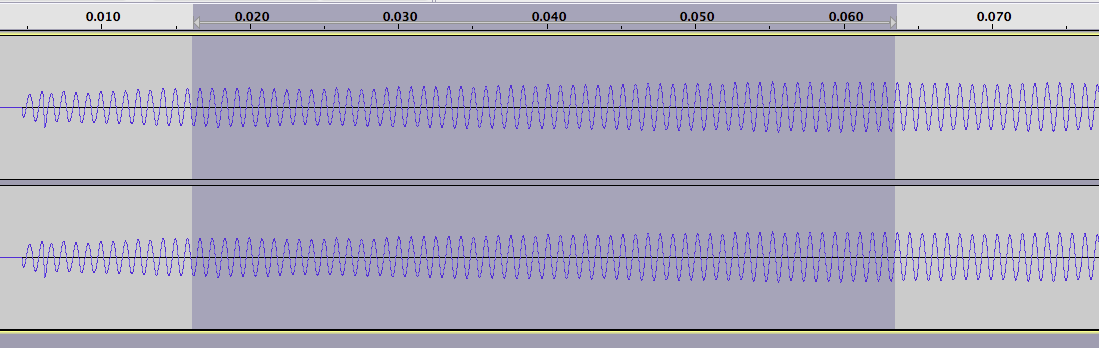
\includegraphics[width=40mm]{figures/whistle_frame_t.png}
   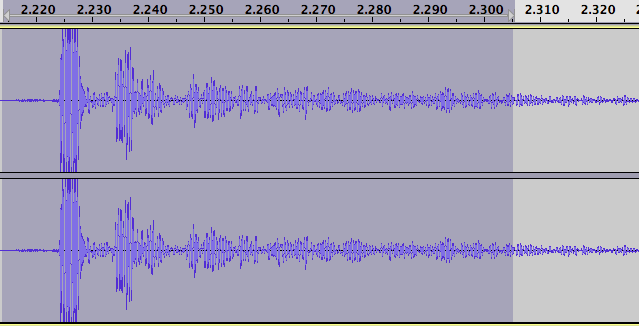
\includegraphics[width=40mm]{figures/snapTimeDomainFrame.png}
   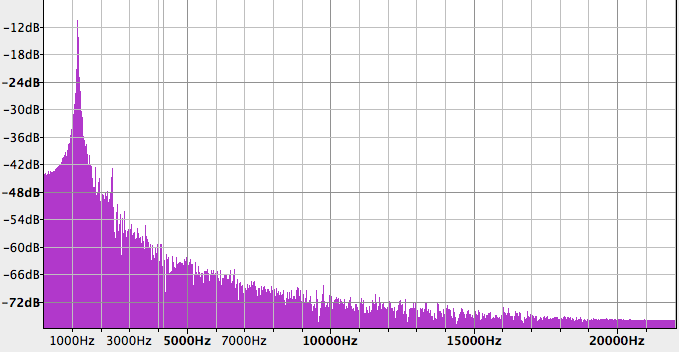
\includegraphics[width=40mm]{figures/whistle_frame_f.png}
   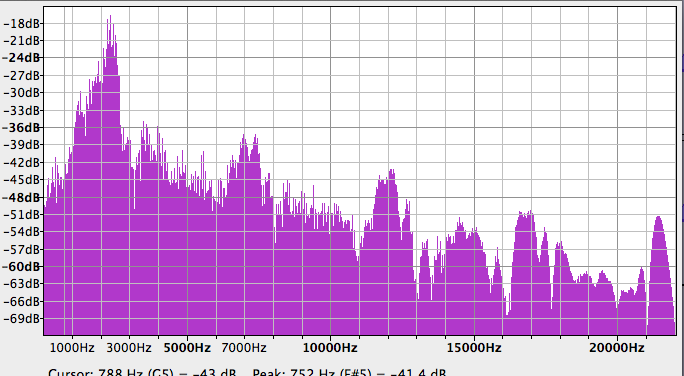
\includegraphics[width=40mm]{figures/SnapFreqDomainFrame.png}
   \caption{The main challenge of the project was generating features to differentiate between these two graphs. (Left: Whistle. Right: Snap); Top: Time Domain. Bottom: Frequency Domain}
   \label{overflow}
   \end{figure}



\subsection{Input}
The WebAudioAPI exposes microphone data sampled at $44,100Hz$. To deal with the constraints specified in Section 2.3, relatively small chunks of sound are processed at a time. The two main parameters of the Input Process is the \textbf{Frame Size} and the \textbf{Hop Size}.
\begin{figure}[h]
\centering
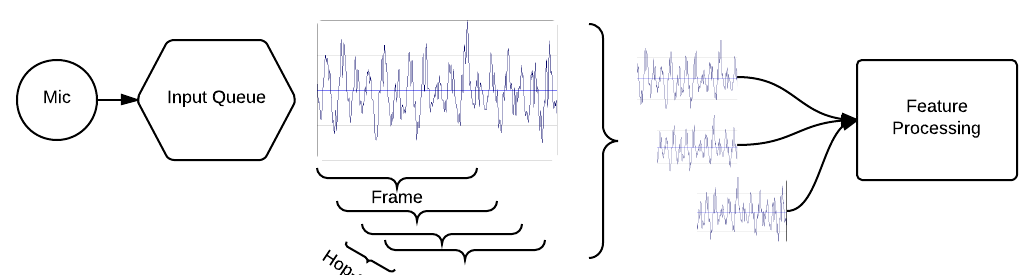
\includegraphics[width=80mm]{figures/InputDiagram.png}
\caption{The input process queue. The sample is retrieved by a window which is moved by a ``hop size'' every iteration.}
\label{overflow}
\end{figure}

The frame size specifies the size the PCM array we will process in a local context for features. Currently the project uses a frame size of 2048 samples. At this sample rate, 2048 samples is equivalent to $46ms$ of sound.
\par The hop size is the distance the frame is moved when processing the next frame. When the hop size is less than the frame size, portions of samples are reprocessed. The project currently uses a hop size of 256 values, or 5.8ms. Currently, after processing the 2048 values in the frame the first 256 are discarded and 256 more value are appended to the end from the queue. \par I define a new term \textbf{Safe Feature Width}, which is the largest guaranteed feature size that will be processed in a single frame:

\begin{align}
   SFW = WindowFrame - HopSize
\end{align}

Currently, in the project, the SFW is approximately 40ms.

\subsection{Feature Generation}


The input queue passes frames of sound data to the Feature Generator. First the sound frame is processed temporally in the Time Domain (no FFT). The temporal processor has the option to normalize the sound sample. If normalization is selected, a \textbf{Peak Normalization} algorithm is used. This algorithm simply scales all PCM values so that maximum value is equal to some target maximum. The project currently normalizes the maximum value to be $0.3$. Peak normalization gives the benefit that it makes peak analysis more resistant to varying whistle volumes.
\par Next the sample is processed in the Frequency domain. The Spectral Processor performs a FFT on the audio frame, and then attaches a set of spectral features.

\par The following sections contain the current temporal and spectral features generated on a local sample. All algorithms were custom implemented in JavaScript and can be found in SoundMath.js, SpectralProcessor.js, and TemporalProcessor.js. Many algorithms are used for both the the Time Domain and Frequency Domain. In this case I will only describe them in the Temporal section, and refer the reader to the appropriate subsection in the Spectral section.


\subsubsection{Temporal Features and Relevant Methods}
\subsubsection {Energy}
   The power of a sound signal is defined as:
   \begin{align}
      p_x(n) = |x(n)|^2
   \end{align}
   The energy of a sound signal is defined as:
   \begin{align}
     Energy = \sum_{n=0}^N p_x(n)
   \end{align}
   Therefore, four features attached to a signal that can be computed in $O(n)$ time is the \textbf{total energy} of the signal, the \textbf{maximum power} and \textbf{average power} and the \textbf{power spread} of a signal.

   \subsubsection {Envelope Analysis}
   Envelope Analysis is currently done through a heuristic which identifies high and medium peaks in the representation of the sound using a Peak Detection routine. These peaks can then be analyzed. One current measure computes the flatness of the envelope.
    \subsubsection {Peak Detection}
    Peaks are found with a routine that takes the following parameters:
      \begin{itemize}
        \item Number of left and right neighbors the inspected value must exceed to be a peak
        \item Sensitivity - an \textbf{amount} by which the current value must exceed its neighbors by to be a peak (default: 0)
        \item Threshold - a base level which the current value must clear to be a peak (default: 0)
      \end{itemize}
   \subsubsection{Flatness}
      Flatness is a measure of how ``spiky'' on envelope is. A flat envelope will have a flatness of 1, while a peaked envelope will have a flatness closer to zero. The flatness is the ratio of the geometric and arithmetic means of the data.
      \begin{align}
      Flatness = \frac{exp(\frac{1}{N}\sum_{n=0}^{N-1}lnx(n))}{\frac{1}{N}\sum_{n=0}^{N-1}x(n)}
      \end{align}
   \subsubsection{Effective Duration}
      Effective duration is the amount of time a signal has power above a certain threshold. In this project I used the mean power as the threshold. Percussive sounds typically have small effective durations and sustained have higher effective durations.
   \subsubsection{Percussive Partition}
   \begin{lstlisting}
   PercussivePartition(partitionSize)
      return subarray with maximum energy
   \end{lstlisting}

   Inspired by creating a method to identify sounds with percussive spikes (like a snap) the percussive partition routine finds a contiguous subsection of the array with the maximum energy. This array can subsequently be processed in the Spectral domain. This isolates the sample from white noise pollution such as the background or simultaneous sustained whistle.

   \subsubsection{Percussive Percent}
   The percussive percent is the total energy of the Percussive Partition total divided by the total energy of the sample:
    \begin{align}
      \frac{TotalEnergy(PercussivePartition(signal))}{ TotalEnergy(signal)}
   \end{align}
   Expectedly, percussive sounds typically have very high percussive percents.

\subsubsection{Spectral Features and Relevant Methods}
The following sections describe the features generated on the result of the FFT of the signal.
   \subsubsection{Spectral Envelope}
   Again, the Peak Finding routine is run on the FFT information to find the spectral envelope. See Peak Detection and Envelope Analysis in the Temporal Feature section for more information.
   \subsubsection{Max Frequency}
   The max frequency is simply the frequency value with largest magnitude. This is very important for whistle detection.
   \subsubsection{Spectral Centroid}
   The Spectral centroid is the weighted average frequency of the spectrum, where the weights are the amplitudes of the frequencies:
   \begin{align}
      \sum_{n=0}^{N-1} \frac{frequencyBucket(n)*f(n)}{frequencyBucket(n)}
   \end{align}
    \subsubsection{Spectral Spread}
    The spectral spread is simply the weighted spread of frequency values around the spectral centroid.
     \begin{align}
    \sum_{n=0}^{N-1} \frac{(spectralCentroid-spectralBucket(n)*f(n))^2}{frequencyBucket(n)}
    \end{align}
\subsection{Spectral Slope}
   The spectral slope is the least squares linear regression calculated on the spectral envelope.



\subsection{Feature Matcher and Output}
The Feature Matcher has two main routines. Calculate local similarity, and calculate global similarity. This routine only occurs if the signal passes some minimum energy threshold. This is to prevent finding random events in white noise. The user of the library has the option to define functions that will score the local and optional global similarity of the features to whistles and snaps, and the weights used applied to those scores before the value is compared to a final decision threshold. This design was inspired by the perceptron model used in Neural Networking.


\begin{figure}[h]
   \centering
   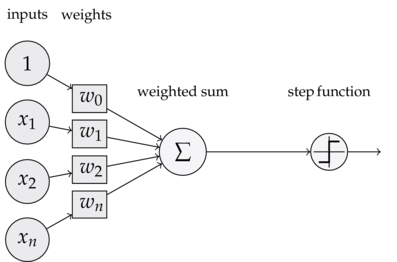
\includegraphics[width=80mm]{figures/perceptronmodel.png}
   \caption{The perceptron model inspired the design of the feature matcher. The current engine uses a binary perceptron.}
   \label{overflow}
\end{figure}


\par As noted, the Feature Matcher has a global similarity component. It allows this through a history of the last $n$ decisions and samples. Currently, the global component is only used to limit the number of events emitted for a snap. Due to the small hop size, a signal snap will be processed multiple times, thus, a snap event is only emitted if the last five history samples do not contain a snap event.

\par  I currently use a method that has perceptrons that heavily punish for features that do not meet the expected set of features of a whistle and snap. Essentially, it preforms a binary check of features - and an event is produced if and only if all test are passed.  However, the architecture allows for a more robust similarity test, that factors in the degree of similarity and can include feature weights. This is possible with the perceptron model or other normalized feature vector distance methods, such as term frequency-inverse document frequency.

\begin{figure}[h]
   \centering
   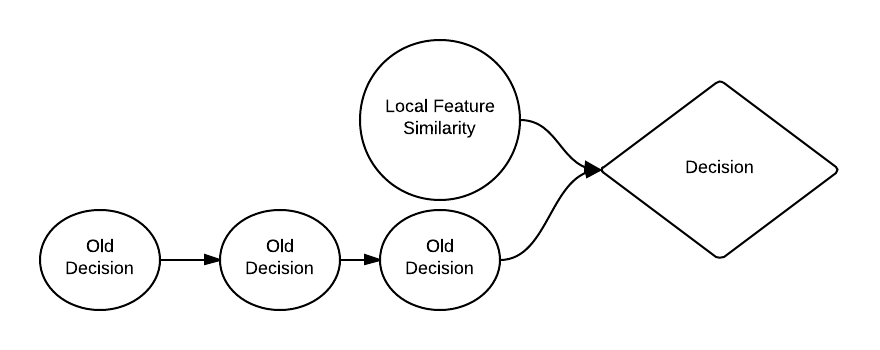
\includegraphics[width=80mm]{figures/FeatureMatcherFuture.png}
   \caption{The feature matcher allows both local similarity and a small amount of global context through access to history of previous decisions.}
   \label{overflow}
\end{figure}

\section{Results}
   The Feature Generator in the project attaches a sizable number of features to a sound sample, most in linear time,  (a very small computational foot print). However, mostly accurate classification can actually be accomplished with very few of these features. In future work, the feature generator may have even more algorithms to calculate features, but the features will be calculated only if they are used in the matcher. This section discusses the result of running the feature generator on test whistles and snaps, and the selection of good features to differentiate whistles and snaps.

   \subsection{Features of Whistles}

   Figure 15 shows one frame of a steady whistle in the both in the time domain and frequency domain. The whistle has a relatively constant temporal envelop. This is because most people whistle at a constant volume. Thus, this results in it having a \textbf{effective duration} greater than $0.3$. (Note the maximum Effective duration is $0.5$).  A similar test used \textbf{temporal flatness}. Most whistles had a temporal flatness above $0.9$, however, a threshold of $0.7$ was used to allow for whistles that change volume to still be accepted.
   \par However, most of the useful whistle features are found in the frequency domain. A whistle has a single characteristic peak in the frequency domain at its pitch. Thus, The vast majority of its spectral content is also between $0$ and $5000$Hz. Thus, the \textbf{spectral spread} was another filter. Any signal with a spectral standard deviation greater than 2000hz was heavily penalized. It is clear that whistles frequency content is much more compact than a snap's frequency content.

   \par Next, the spectral envelope was analyzed. A high peak threshold was set so that whistles should only have one ``high peak'' value in the envelope. If a single high peak was detected, the frequency value of the peak was confirmed to be in an acceptable frequency range of $700$Hz and $3500$Hz. This is lower than Nilsson's range, but I found it to be a bit more practical for the average whistler. Again, my perceptron model was essentially a boolean filter. The following list summarizes the filters I currently use for whistle detection:
    \begin{itemize}
        \item Effective duration $> 0.3$
        \item Temporal Flatness  $>0.7$
        \item Single ``High'' peak
        \item Peak frequency between $700$ and $3500$Hz
        \item Spectral standard deviation less than $2000$
      \end{itemize}

   \begin{figure}[h]
   \centering
   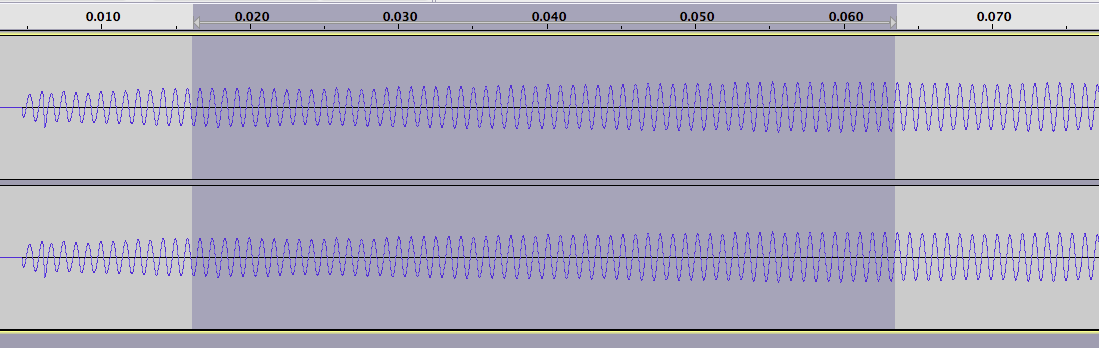
\includegraphics[width=80mm]{figures/whistle_frame_t.png}
   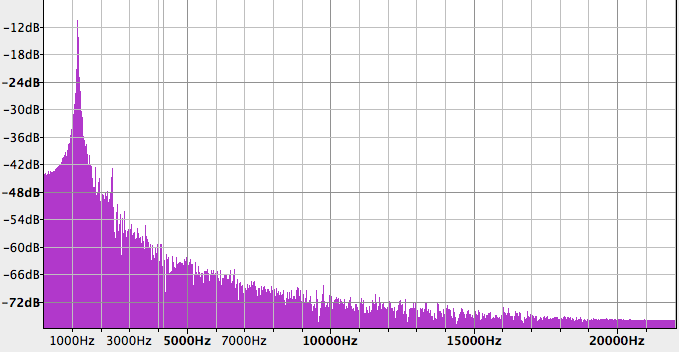
\includegraphics[width=80mm]{figures/whistle_frame_f.png}
   \caption{A 40ms frame of whistle data at attempted constant pitch.}
   \label{overflow}
   \end{figure}
   \par
   These features identified whistles with accuracy above 95\% on the sample sound files. Whistles of all volumes and rapidly changing pitches all were successfully identified. The system does fire false positives. However, this usually only occurs when the ambient noise has a clear pitch. For example, play the ``indie music" on Whistle Hero. The only time a whistle event occurs (the white marker dot moves) is when there is actually whistling in the song, or the song contains strong tonal vocals. Also, when I was testing the game, and a train whistle would sound - the game would pick this up as input. This is an inherent limitation of using sound as input.

   \subsection{Features of Snaps}

   Snaps, and other percussive sounds, are notably characterized by a huge spike of energy in the time domain. Thus, the first feature the boolean-perceptron for snap detection uses is a temporal flatness less then $0.5$. (The vast majority of snaps have a flatness score $<0.1$). Next, a percussive percent of greater than $0.7$. These filters work very well at detecting any percussive sound. Thus, clapping works just as well as snaps as input.

     \begin{figure}[h]
   \centering
   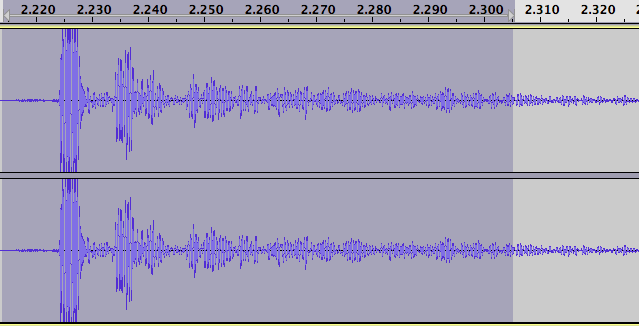
\includegraphics[width=80mm]{figures/snapTimeDomainFrame.png}
   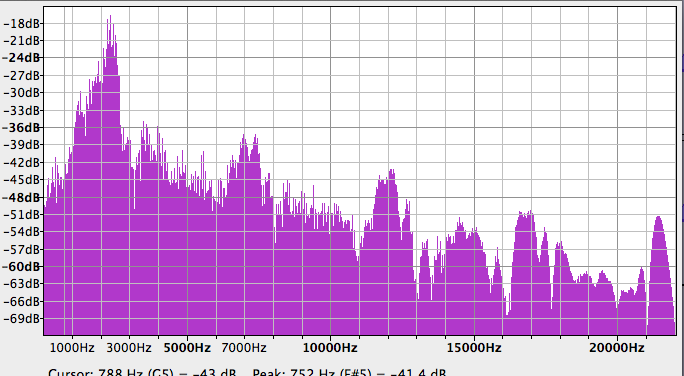
\includegraphics[width=80mm]{figures/SnapFreqDomainFrame.png}
   \caption{A 40ms frame of a snap. }
   \label{overflow}
   \end{figure}

   \par
   The frequency domain is where it may be possible to separate snaps from claps. I did find snaps to have a consistent spectral shape, but could not figure out the best mathematical method to differentiate it from other percussive sounds. Thus, I aimed to use spectral filters to remove percussive \textit{whistles}, as the input engine would fail if whistle events ever also registered as snaps. Thus, I required a spectral standard deviation greater than 2000 (again, the spectral shape of snaps is much more spread out than whistles). Finally, I required that the spectral envelope had no high peaks similar to a whistle.


   \begin{figure}[h]
   \centering
   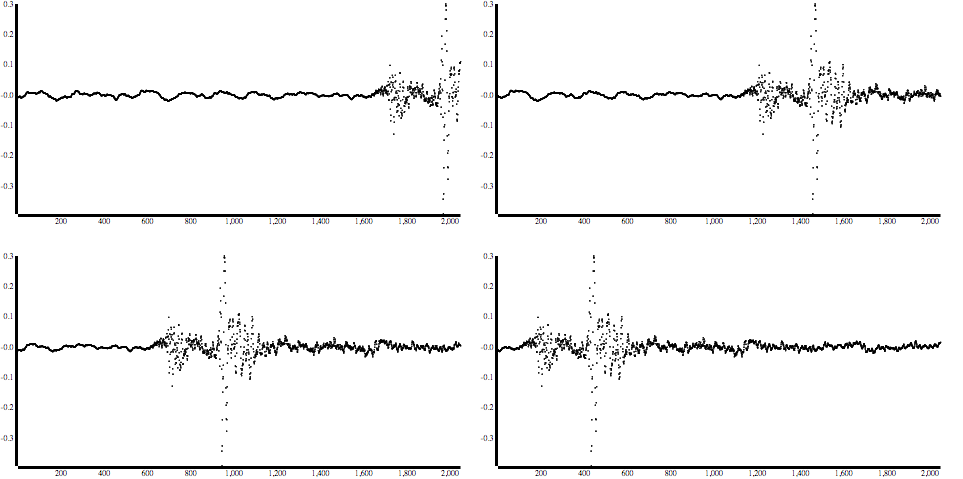
\includegraphics[width=80mm]{figures/projectplot}

   \caption{Plot of a real user's snap passing through the Feature Matcher in Time Domain. Plots generated by quickplot.js and D3.js. The energy spike is apparent. }
   \label{overflow}
   \end{figure}

   \par
   Loud, ``poppy'', snaps are recognized with greater than 95\% accuracy. However, people often are not able to snap clearly. Instead their snaps are soft and muted. In the final version of the project, I have adjusted some of the perceptron filters to be more lenient towards soft snaps, by attempting to filter out the ambient environment noise to boost the percussive percent of samples with an overall low energy content (a quiet snap used to be penalized in the percussive percent algorithm because ambient noise made up a large part of its signal). Figure 17, shows the graphical analyzing software I used to help visualize what was passing through the feature generator with snaps.
   \par Weaker snaps are recognized with greater than 80\% accuracy in the test files. However, in practice, my snaps are not recognized frequently enough so that game play is slightly frustrating. Also, the loosening of the filter constraints allows many false positives. For example, play the ``rock'' music in Whistle Hero. Nearly every beat of the bass drum registers as a percussive snap event. So long as users are wearing headphones, this is not a huge problem, as ambient noise rarely contains percussive sound.



\section{Discussion}
   \subsection{Using the API}
      Using the API is as simply as listening for ``SoundInput.detect'' events. You can then switch on the type of input event, and get more details if they exist. Thus, if work is continued on the detection methods, games won't have to change any of their code - they will just work better.
   \subsection{Whistle Hero}
   Whistle Hero is demonstration of the API. It assumes no knowledge of how the Audio Processing works besides listening and reacting to snaps and whistles. In the game, a user attempts to ``paint'' a series of bar sliding across three different bands. The user whistles high to move a white dot which will activate the band it rests in. When the bars overlap the active band, the user snaps her fingers or claps to paint the bar. More points are rewarded for entirely painting the bar. Points are lost if the user does not paint any portion of a bar.

    \begin{figure}[h]
   \centering
   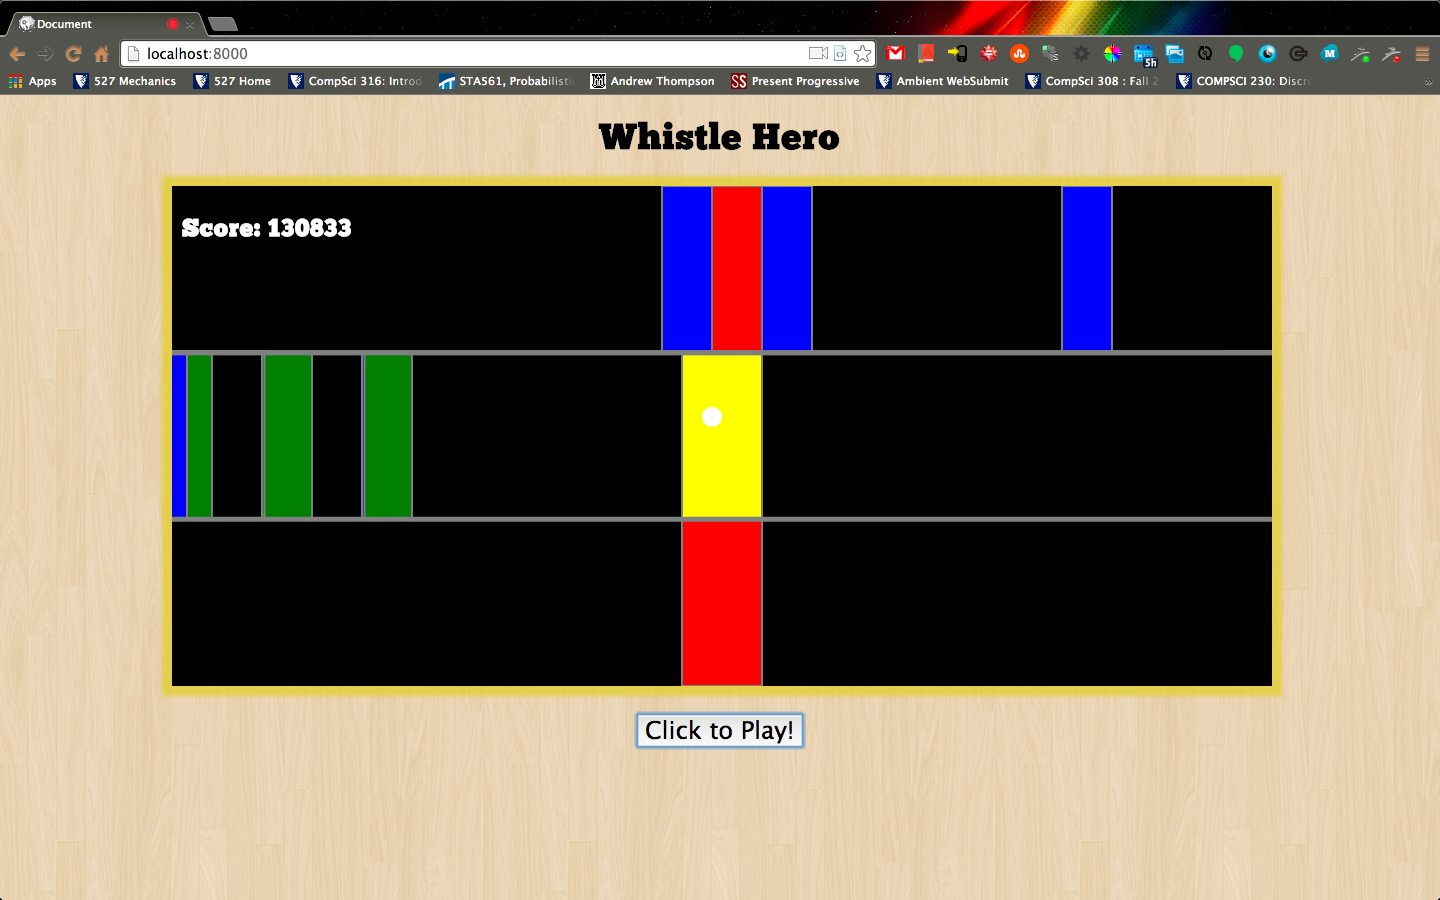
\includegraphics[width=80mm]{figures/whistlehero.png}
   \caption{Whistle Hero. A sample game made with the Sound API.}
   \label{overflow}
   \end{figure}

   \par A prototype of the game is on \textbf{benschwab.github.io}, but the notes have not been optimized to match the songs. It would be feasible for a developer to create bar patterns which match the pitch and beat of the song.

\section{Conclusion}
   Entering this project I had not been exposed to the FFT or signal processing in my education. Initially, I planned to do more mathematically intensive signal processing in the project, however, the restraints of a Game Engine restricted the set of signal algorithms to those that could run in less than $O(n*log(n))$ time. The current set of features work very well for whistles, but not as well for snaps that are not perfectly clear. For most of my friends, clapping was a more consistent method of producing a percussive. If more input events where to be specified, the project would have to uses stronger features to differentiate between events. In particular, more work could be done in the spectral domain, such as envelop convolution as a test of similarity.
   \subsection{Future Work}
   \subsubsection{Necessary Feature Specification}
  If the project gains more features, it may become computationally infeasible to calculate all of them. Thus, the user will be able to specify what features the Matcher will use. The Generator will only produce those features, significantly reducing the computational complexity.
   \subsubsection{Automatic Training}
   With marginal extra effort, I could allow a user to send a set of Sound Samples to train the input engine on. This would run the samples through the Feature Generator, and determine average features. However, this would require the Feature Matcher to have a solid implementation of an automated TF-IDF weighting of features, as much of my work was figuring out how to optimally weight features for snaps and whistles. Whether or not this could be generated automatically would require further research.
   \subsubsection{Better use of ST-FFT}
   Currently the project has the infrastructure to support the use of Short-Term Fast Fourier Transform. (See section 4.1). However, I currently the result  of short-time FFT to the Spectral processor by itself. Alternatively, I could send an entire matrix of short-time FFTs. This matrix would thus add the dimension of time. This would allow algorithms that analyzes samples simultaneously in the frequency and time domains. Due to the percussive nature of snaps, this would likely lead to useful differentiating features.

%----------------------------------------------------------------------------------------
%  REFERENCE LIST

\begin{thebibliography}{99} % Bibliography - this is intentionally simple in this template


\bibitem[Nilsson, 2008]{Nilsson:2008dg}
Nilsson, Bartunek, Nordberg, Claesson. Blekinge Institue of Technology
\newblock {\em Human Whistle Detection and Frequency Estimation}

\bibitem[Peeters, 2004]{Peeters:2004dg}
Peeters. Ircam, Analysis/Syntehsis Team, Igor Stravinksy.
\newblock {\em A large set of audio features for sound description (similarity and classification) in the CUIDADO project}

\bibitem[Sauer, 2012]{Sauer:2006dg}
Sauer, Numerical Analysis 2nd ed. Pearson Education, Inc.
\newblock {\em The Fourier Transform}, p468--499.

\bibitem[Schwarz, 1998]{Schwarz:1998dg}
Diemo Schwarz, Institu de la Recherche et Coordination Acoustique
\newblock {\em Spectral Envelopes in Sound Analysis and Synthesis}

\bibitem[Smus, 2013]{Smus:2013dg}
Smus, Boris. Web Audio API O'Reilly Media, Inc.
\newblock {\em Fundamentals, Advanced Topics}


\end{thebibliography}

%----------------------------------------------------------------------------------------

\end{document}